\section{\Sys Design}
\label{sec:methodology}

\Sys, depicted in Figure \ref{arch}, comprises four key modules: a provenance graph constructor, a Semantic Vectors Harmonization, Federated Learning Module, and Anomaly Detection. The main server is responsible for initiating the global model weights, which are then transmitted to the client machines. The clients use these weights as their starting point and conduct model training on their respective local datasets. Subsequently, the clients send their updated weights back to the main server for federated averaging.

In addition to the primary task, each client machine also trains a word2vec model to feature semantic attributes in audit logs. It's noteworthy that the word2vec models on different clients may yield distinct embeddings for the same tokens. To address this potential non-iid data problem, \Sys employs the utility server to harmonize these models.

\subsection{Provenance Graph Constructor}
Our approach starts by converting system logs into provenance graphs through a three-step process. Initially, the system, \Sys, processes system logs like Windows Event Logs or Linux Audit Logs, which are composed of host event details including process activities, file interactions, and network engagements. \Sys works with batches of audit logs, utilizing a sliding window technique to create the provenance graph. This graph consists of two kinds of nodes: process nodes and object nodes. The object nodes represent various system entities such as files, network streams, modules, and other system components. The connections between these nodes are marked with labels indicating the event type, elucidating the cause-and-effect relationship among the connected nodes and the event's timestamp. Additionally, these nodes are equipped with attributes like process identifiers, command lines, file paths, IP addresses, port details, and module paths, offering additional insights and specifics.

\subsection{Semantic Vectors Harmonization}

\subsection{Federated Learning Module}

\subsection{Anomaly Detection}


\begin{figure}[t!]
    \centering
    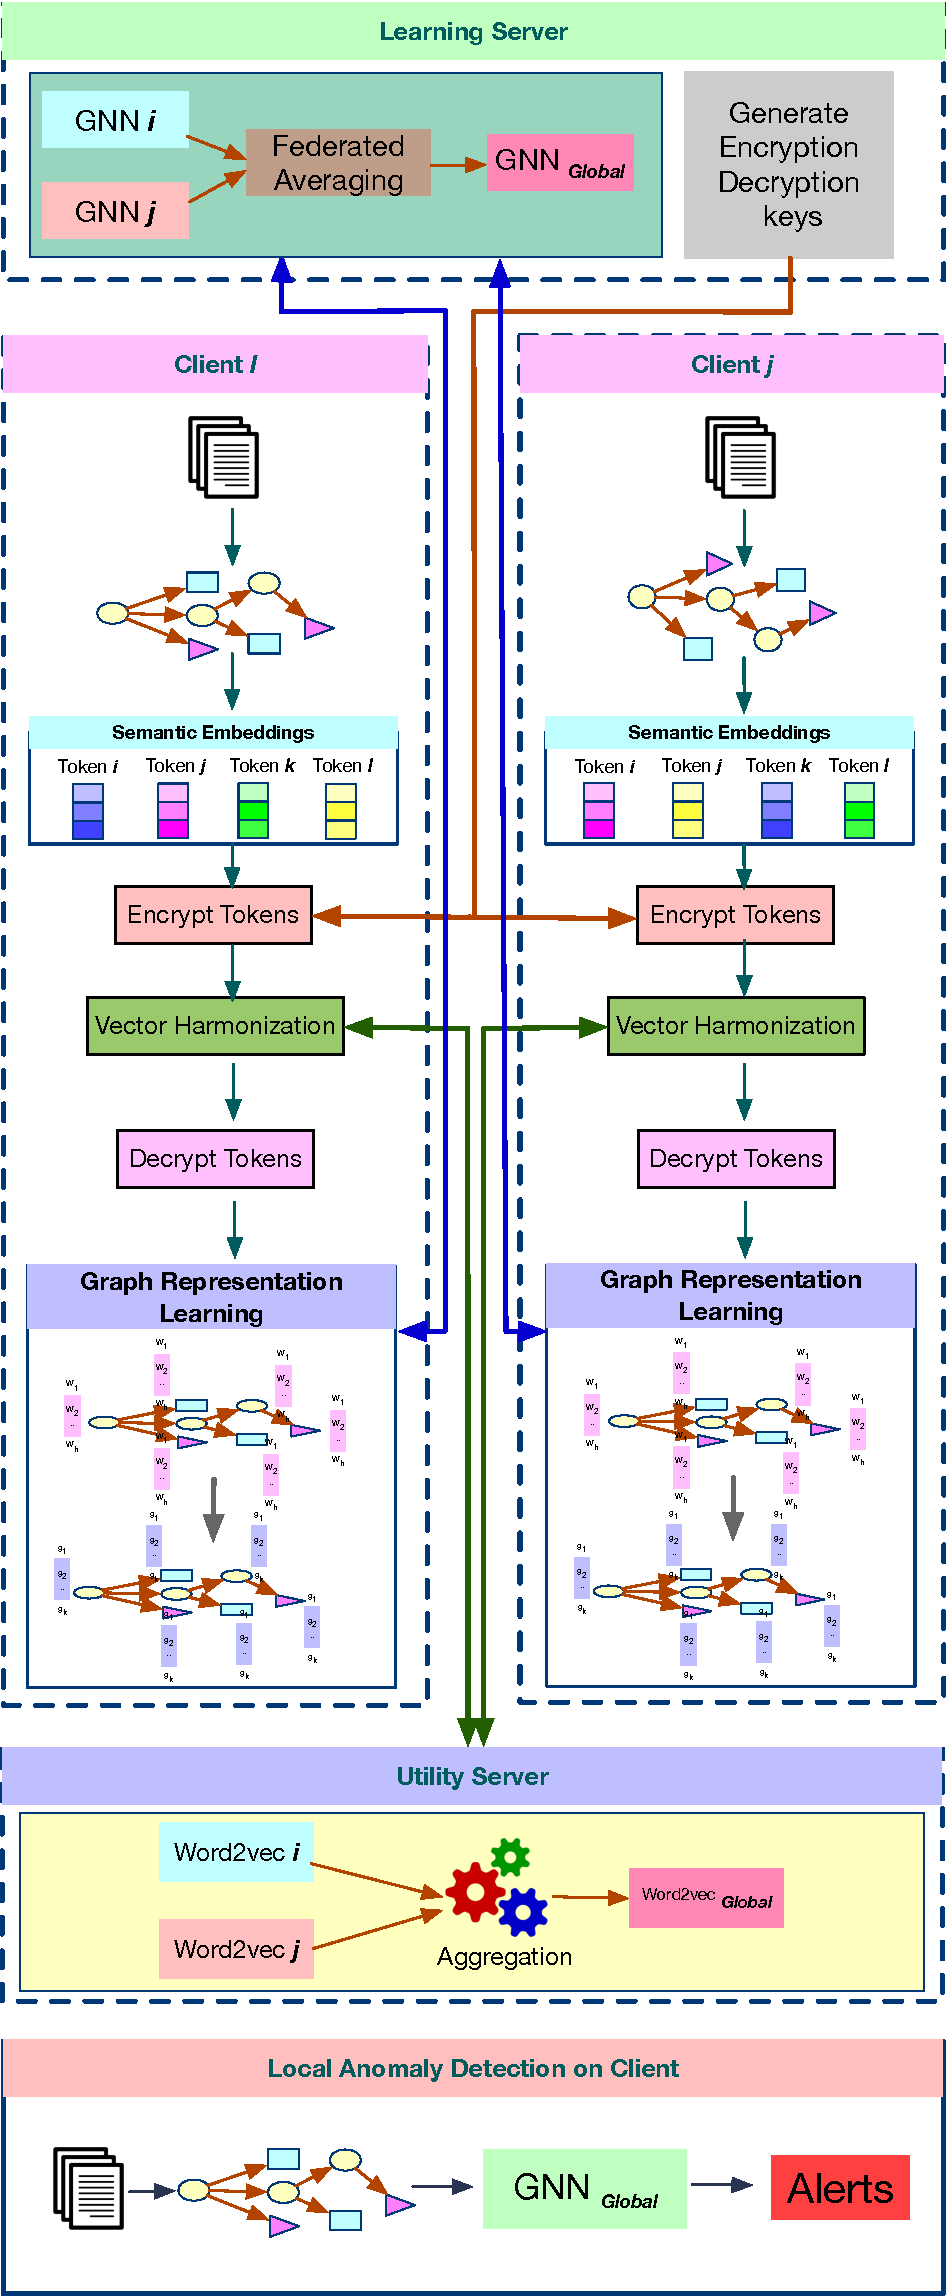
\includegraphics[width=0.45\textwidth]{fig/arch.pdf}
    \caption{High Level Architecture of \Sys}
    \vspace{-3ex}
    \label{arch}
  \end{figure}
